\documentclass[a4paper,10pt,ngerman]{scrartcl}
\usepackage{babel}
\usepackage[T1]{fontenc}
\usepackage[utf8x]{inputenc}
\usepackage[a4paper,margin=2.5cm,footskip=0.5cm]{geometry}

% Die nächsten drei Felder bitte anpassen:
\newcommand{\Aufgabe}{Aufgabe 1: Weniger krumme Touren} % Aufgabennummer und Aufgabennamen angeben
\newcommand{\TeilnahmeId}{64609}                  % Teilnahme-ID angeben
\newcommand{\Name}{Richard Ewert}             % Name des Bearbeiter / der Bearbeiterin dieser Aufgabe angeben


% Kopf- und Fußzeilen
\usepackage{scrlayer-scrpage, lastpage}
\setkomafont{pageheadfoot}{\large\textrm}
\lohead{\Aufgabe}
\rohead{Teilnahme-ID: \TeilnahmeId}
\cfoot*{\thepage{}/\pageref{LastPage}}

% Position des Titels
\usepackage{titling}
\setlength{\droptitle}{-1.0cm}


% Für mathematische Befehle und Symbole
\usepackage{amsmath}
\usepackage{amssymb}

% Für Bilder
\usepackage{graphicx}

% Für Algorithmen
\usepackage{algpseudocode}

% Für Quelltext
\usepackage{listings}
\usepackage{color}
%\definecolor{mygreen}{rgb}{0,0.6,0}
%\definecolor{mygray}{rgb}{0.5,0.5,0.5}
%\definecolor{mymauve}{rgb}{0.58,0,0.82}
%\lstset{
%  keywordstyle=\color{blue},commentstyle=\color{mygreen},
%  stringstyle=\color{mymauve},rulecolor=\color{black},
%  basicstyle=\footnotesize\ttfamily,numberstyle=\tiny\color{mygray},
%  captionpos=b, % sets the caption-position to bottom
%  keepspaces=true, % keeps spaces in text
% numbers=left, numbersep=5pt, showspaces=false,showstringspaces=true,
% showtabs=false, stepnumber=2, tabsize=2, title=\lstname
%}
\lstdefinelanguage{Javascript}{ % JavaScript ist als einzige Sprache noch nicht vordefiniert
  keywords={break, case, catch, continue, debugger, default, delete, do, else, finally, for, function, if, in, instanceof, new, return, switch, this, throw, try, typeof, var, void, while, with},
  morecomment=[l]{//},
  morecomment=[s]{/*}{*/},
  morestring=[b]',
  morestring=[b]",
  sensitive=true
}
%Taken from: ttps://github.com/denki/listings-rust/blob/master/listings-rust.sty
\lstdefinelanguage{Rust}{%
  sensitive%
, morecomment=[l]{//}%
, morecomment=[l]{///}%
, morecomment=[s]{/*}{*/}%
, moredelim=[s][{\itshape\color[rgb]{1,1,0.75}}]{\#[}{]}%
, morestring=[b]{"}%
, alsodigit={}%
, alsoother={}%
, alsoletter={!}%
%
%
% [1] reserve keywords
% [2] traits
% [3] primitive types
% [4] type and value constructors
% [5] identifier
%
, morekeywords={break, continue, else, for, if, in, loop, match, return, while, let}  % control flow keywords
, morekeywords=[3]{as, const, move, mut, ref, static, *, &}  % in the context of variables
, morekeywords={dyn, enum, fn, impl, Self, self, struct, trait, type, union, use, where}  % in the context of declarations
, morekeywords={crate, extern, mod, pub, super}  % in the context of modularisation
, morekeywords={unsafe}  % markers
, morekeywords={abstract, alignof, become, box, do, final, macro, offsetof, override, priv, proc, pure, sizeof, typeof, unsized, virtual, yield}  % reserved identifiers
%
% grep 'pub trait [A-Za-z][A-Za-z0-9]*' -r . | sed 's/^.*pub trait \([A-Za-z][A-Za-z0-9]*\).*/\1/g' | sort -u | tr '\n' ',' | sed 's/^\(.*\),$/{\1}\n/g' | sed 's/,/, /g'
, morekeywords=[2]{Add, AddAssign, Any, AsciiExt, AsInner, AsInnerMut, AsMut, AsRawFd, AsRawHandle, AsRawSocket, AsRef, Binary, BitAnd, BitAndAssign, Bitor, BitOr, BitOrAssign, BitXor, BitXorAssign, Borrow, BorrowMut, Boxed, BoxPlace, BufRead, BuildHasher, CastInto, CharExt, Clone, CoerceUnsized, CommandExt, Copy, Debug, DecodableFloat, Default, Deref, DerefMut, DirBuilderExt, DirEntryExt, Display, Div, DivAssign, DoubleEndedIterator, DoubleEndedSearcher, Drop, EnvKey, Eq, Error, ExactSizeIterator, ExitStatusExt, Extend, FileExt, FileTypeExt, Float, Fn, FnBox, FnMut, FnOnce, Freeze, From, FromInner, FromIterator, FromRawFd, FromRawHandle, FromRawSocket, FromStr, FullOps, FusedIterator, Generator, Hash, Hasher, Index, IndexMut, InPlace, Int, Into, IntoCow, IntoInner, IntoIterator, IntoRawFd, IntoRawHandle, IntoRawSocket, IsMinusOne, IsZero, Iterator, JoinHandleExt, LargeInt, LowerExp, LowerHex, MetadataExt, Mul, MulAssign, Neg, Not, Octal, OpenOptionsExt, Ord, OsStrExt, OsStringExt, Packet, PartialEq, PartialOrd, Pattern, PermissionsExt, Place, Placer, Pointer, Product, Put, RangeArgument, RawFloat, Read, Rem, RemAssign, Seek, Shl, ShlAssign, Shr, ShrAssign, Sized, SliceConcatExt, SliceExt, SliceIndex, Stats, Step, StrExt, Sub, SubAssign, Sum, Sync, TDynBenchFn, Terminal, Termination, ToOwned, ToSocketAddrs, ToString, Try, TryFrom, TryInto, UnicodeStr, Unsize, UpperExp, UpperHex, WideInt, Write}
, morekeywords=[2]{Send}  % additional traits
%
, morekeywords=[3]{bool, char, f32, f64, i8, i16, i32, i64, isize, str, u8, u16, u32, u64, unit, usize, i128, u128}  % primitive types
%
, morekeywords=[4]{Err, false, None, Ok, Some, true}  % prelude value constructors
% grep 'pub \(type\|struct\|enum\) [A-Za-z][A-Za-z0-9]*' -r . | sed 's/^.*pub \(type\|struct\|enum\) \([A-Za-z][A-Za-z0-9]*\).*/\2/g' | sort -u | tr '\n' ',' | sed 's/^\(.*\),$/{\1}\n/g' | sed 's/,/, /g'    
, morekeywords=[3]{AccessError, Adddf3, AddI128, AddoI128, AddoU128, ADDRESS, ADDRESS64, addrinfo, ADDRINFOA, AddrParseError, Addsf3, AddU128, advice, aiocb, Alignment, AllocErr, AnonPipe, Answer, Arc, Args, ArgsInnerDebug, ArgsOs, Argument, Arguments, ArgumentV1, Ashldi3, Ashlti3, Ashrdi3, Ashrti3, AssertParamIsClone, AssertParamIsCopy, AssertParamIsEq, AssertUnwindSafe, AtomicBool, AtomicPtr, Attr, auxtype, auxv, BackPlace, BacktraceContext, Barrier, BarrierWaitResult, Bencher, BenchMode, BenchSamples, BinaryHeap, BinaryHeapPlace, blkcnt, blkcnt64, blksize, BOOL, boolean, BOOLEAN, BoolTrie, BorrowError, BorrowMutError, Bound, Box, bpf, BTreeMap, BTreeSet, Bucket, BucketState, Buf, BufReader, BufWriter, Builder, BuildHasherDefault, BY, BYTE, Bytes, CannotReallocInPlace, cc, Cell, Chain, CHAR, CharIndices, CharPredicateSearcher, Chars, CharSearcher, CharsError, CharSliceSearcher, CharTryFromError, Child, ChildPipes, ChildStderr, ChildStdin, ChildStdio, ChildStdout, Chunks, ChunksMut, ciovec, clock, clockid, Cloned, cmsgcred, cmsghdr, CodePoint, Color, ColorConfig, Command, CommandEnv, Component, Components, CONDITION, condvar, Condvar, CONSOLE, CONTEXT, Count, Cow, cpu, CRITICAL, CStr, CString, CStringArray, Cursor, Cycle, CycleIter, daddr, DebugList, DebugMap, DebugSet, DebugStruct, DebugTuple, Decimal, Decoded, DecodeUtf16, DecodeUtf16Error, DecodeUtf8, DefaultEnvKey, DefaultHasher, dev, device, Difference, Digit32, DIR, DirBuilder, dircookie, dirent, dirent64, DirEntry, Discriminant, DISPATCHER, Display, Divdf3, Divdi3, Divmoddi4, Divmodsi4, Divsf3, Divsi3, Divti3, dl, Dl, Dlmalloc, Dns, DnsAnswer, DnsQuery, dqblk, Drain, DrainFilter, Dtor, Duration, DwarfReader, DWORD, DWORDLONG, DynamicLibrary, Edge, EHAction, EHContext, Elf32, Elf64, Empty, EmptyBucket, EncodeUtf16, EncodeWide, Entry, EntryPlace, Enumerate, Env, epoll, errno, Error, ErrorKind, EscapeDebug, EscapeDefault, EscapeUnicode, event, Event, eventrwflags, eventtype, ExactChunks, ExactChunksMut, EXCEPTION, Excess, ExchangeHeapSingleton, exit, exitcode, ExitStatus, Failure, fd, fdflags, fdsflags, fdstat, ff, fflags, File, FILE, FileAttr, filedelta, FileDesc, FilePermissions, filesize, filestat, FILETIME, filetype, FileType, Filter, FilterMap, Fixdfdi, Fixdfsi, Fixdfti, Fixsfdi, Fixsfsi, Fixsfti, Fixunsdfdi, Fixunsdfsi, Fixunsdfti, Fixunssfdi, Fixunssfsi, Fixunssfti, Flag, FlatMap, Floatdidf, FLOATING, Floatsidf, Floatsisf, Floattidf, Floattisf, Floatundidf, Floatunsidf, Floatunsisf, Floatuntidf, Floatuntisf, flock, ForceResult, FormatSpec, Formatted, Formatter, Fp, FpCategory, fpos, fpos64, fpreg, fpregset, FPUControlWord, Frame, FromBytesWithNulError, FromUtf16Error, FromUtf8Error, FrontPlace, fsblkcnt, fsfilcnt, fsflags, fsid, fstore, fsword, FullBucket, FullBucketMut, FullDecoded, Fuse, GapThenFull, GeneratorState, gid, glob, glob64, GlobalDlmalloc, greg, group, GROUP, Guard, GUID, Handle, HANDLE, Handler, HashMap, HashSet, Heap, HINSTANCE, HMODULE, hostent, HRESULT, id, idtype, if, ifaddrs, IMAGEHLP, Immut, in, in6, Incoming, Infallible, Initializer, ino, ino64, inode, input, InsertResult, Inspect, Instant, int16, int32, int64, int8, integer, IntermediateBox, Internal, Intersection, intmax, IntoInnerError, IntoIter, IntoStringError, intptr, InvalidSequence, iovec, ip, IpAddr, ipc, Ipv4Addr, ipv6, Ipv6Addr, Ipv6MulticastScope, Iter, IterMut, itimerspec, itimerval, jail, JoinHandle, JoinPathsError, KDHELP64, kevent, kevent64, key, Key, Keys, KV, l4, LARGE, lastlog, launchpad, Layout, Lazy, lconv, Leaf, LeafOrInternal, Lines, LinesAny, LineWriter, linger, linkcount, LinkedList, load, locale, LocalKey, LocalKeyState, Location, lock, LockResult, loff, LONG, lookup, lookupflags, LookupHost, LPBOOL, LPBY, LPBYTE, LPCSTR, LPCVOID, LPCWSTR, LPDWORD, LPFILETIME, LPHANDLE, LPOVERLAPPED, LPPROCESS, LPPROGRESS, LPSECURITY, LPSTARTUPINFO, LPSTR, LPVOID, LPWCH, LPWIN32, LPWSADATA, LPWSAPROTOCOL, LPWSTR, Lshrdi3, Lshrti3, lwpid, M128A, mach, major, Map, mcontext, Metadata, Metric, MetricMap, mflags, minor, mmsghdr, Moddi3, mode, Modsi3, Modti3, MonitorMsg, MOUNT, mprot, mq, mqd, msflags, msghdr, msginfo, msglen, msgqnum, msqid, Muldf3, Mulodi4, Mulosi4, Muloti4, Mulsf3, Multi3, Mut, Mutex, MutexGuard, MyCollection, n16, NamePadding, NativeLibBoilerplate, nfds, nl, nlink, NodeRef, NoneError, NonNull, NonZero, nthreads, NulError, OccupiedEntry, off, off64, oflags, Once, OnceState, OpenOptions, Option, Options, OptRes, Ordering, OsStr, OsString, Output, OVERLAPPED, Owned, Packet, PanicInfo, Param, ParseBoolError, ParseCharError, ParseError, ParseFloatError, ParseIntError, ParseResult, Part, passwd, Path, PathBuf, PCONDITION, PCONSOLE, Peekable, PeekMut, Permissions, PhantomData, pid, Pipes, PlaceBack, PlaceFront, PLARGE, PoisonError, pollfd, PopResult, port, Position, Powidf2, Powisf2, Prefix, PrefixComponent, PrintFormat, proc, Process, PROCESS, processentry, protoent, PSRWLOCK, pthread, ptr, ptrdiff, PVECTORED, Queue, radvisory, RandomState, Range, RangeFrom, RangeFull, RangeInclusive, RangeMut, RangeTo, RangeToInclusive, RawBucket, RawFd, RawHandle, RawPthread, RawSocket, RawTable, RawVec, Rc, ReadDir, Receiver, recv, RecvError, RecvTimeoutError, ReentrantMutex, ReentrantMutexGuard, Ref, RefCell, RefMut, REPARSE, Repeat, Result, Rev, Reverse, riflags, rights, rlim, rlim64, rlimit, rlimit64, roflags, Root, RSplit, RSplitMut, RSplitN, RSplitNMut, RUNTIME, rusage, RwLock, RWLock, RwLockReadGuard, RwLockWriteGuard, sa, SafeHash, Scan, sched, scope, sdflags, SearchResult, SearchStep, SECURITY, SeekFrom, segment, Select, SelectionResult, sem, sembuf, send, Sender, SendError, servent, sf, Shared, shmatt, shmid, ShortReader, ShouldPanic, Shutdown, siflags, sigaction, SigAction, sigevent, sighandler, siginfo, Sign, signal, signalfd, SignalToken, sigset, sigval, Sink, SipHasher, SipHasher13, SipHasher24, size, SIZE, Skip, SkipWhile, Slice, SmallBoolTrie, sockaddr, SOCKADDR, sockcred, Socket, SOCKET, SocketAddr, SocketAddrV4, SocketAddrV6, socklen, speed, Splice, Split, SplitMut, SplitN, SplitNMut, SplitPaths, SplitWhitespace, spwd, SRWLOCK, ssize, stack, STACKFRAME64, StartResult, STARTUPINFO, stat, Stat, stat64, statfs, statfs64, StaticKey, statvfs, StatVfs, statvfs64, Stderr, StderrLock, StderrTerminal, Stdin, StdinLock, Stdio, StdioPipes, Stdout, StdoutLock, StdoutTerminal, StepBy, String, StripPrefixError, StrSearcher, subclockflags, Subdf3, SubI128, SuboI128, SuboU128, subrwflags, subscription, Subsf3, SubU128, Summary, suseconds, SYMBOL, SYMBOLIC, SymmetricDifference, SyncSender, sysinfo, System, SystemTime, SystemTimeError, Take, TakeWhile, tcb, tcflag, TcpListener, TcpStream, TempDir, TermInfo, TerminfoTerminal, termios, termios2, TestDesc, TestDescAndFn, TestEvent, TestFn, TestName, TestOpts, TestResult, Thread, threadattr, threadentry, ThreadId, tid, time, time64, timespec, TimeSpec, timestamp, timeval, timeval32, timezone, tm, tms, ToLowercase, ToUppercase, TraitObject, TryFromIntError, TryFromSliceError, TryIter, TryLockError, TryLockResult, TryRecvError, TrySendError, TypeId, U64x2, ucontext, ucred, Udivdi3, Udivmoddi4, Udivmodsi4, Udivmodti4, Udivsi3, Udivti3, UdpSocket, uid, UINT, uint16, uint32, uint64, uint8, uintmax, uintptr, ulflags, ULONG, ULONGLONG, Umoddi3, Umodsi3, Umodti3, UnicodeVersion, Union, Unique, UnixDatagram, UnixListener, UnixStream, Unpacked, UnsafeCell, UNWIND, UpgradeResult, useconds, user, userdata, USHORT, Utf16Encoder, Utf8Error, Utf8Lossy, Utf8LossyChunk, Utf8LossyChunksIter, utimbuf, utmp, utmpx, utsname, uuid, VacantEntry, Values, ValuesMut, VarError, Variables, Vars, VarsOs, Vec, VecDeque, vm, Void, WaitTimeoutResult, WaitToken, wchar, WCHAR, Weak, whence, WIN32, WinConsole, Windows, WindowsEnvKey, winsize, WORD, Wrapping, wrlen, WSADATA, WSAPROTOCOL, WSAPROTOCOLCHAIN, Wtf8, Wtf8Buf, Wtf8CodePoints, xsw, xucred, Zip, zx, std, cmp, node_mod, Node, Task, input_output_mod, log, MAX, Less, Equal, Greater}
%
, morekeywords=[5]{assert!, assert_eq!, assert_ne!, cfg!, column!, compile_error!, concat!, concat_idents!, debug_assert!, debug_assert_eq!, debug_assert_ne!, env!, eprint!, eprintln!, file!, format!, format_args!, include!, include_bytes!, include_str!, line!, module_path!, option_env!, panic!, print!, println!, select!, stringify!, thread_local!, try!, unimplemented!, unreachable!, vec!, write!, writeln!, debug!, info!, warn!}  % prelude macros
, morekeywords=[6]{render, read_nodes, give_status_info, enumerate, iter, len, push, pop, sort_by, contains, reatain, get_tasks, sort_tasks, solve, append, is_empty, main, init, render, elapsed, as_secs_f32, unwrap, clone, copy, calc_angles_distances, sort_tasks, generate_start_tasks, path_len, indices_to_nodes, now, collect, round, as_micros, solve_recursive, spawn, drop, current, generate_start_paths, new}%functions
}%

\lstdefinestyle{colouredRust}%
{ basicstyle=\ttfamily\color[rgb]{0.9, 0.9, 0.9}%
, identifierstyle=%
, commentstyle=\color[rgb]{0.9, 0.9, 0.5}%
, stringstyle=\color[rgb]{1.0, 0.1, 0.1}%
, keywordstyle=\bfseries% reserved keywords
, keywordstyle=[1]\color[rgb]{0.9,0.3, 0.9}
, keywordstyle=[2]\color[rgb]{0.75, 0, 0}% traits
, keywordstyle=[3]\color[rgb]{0.3, 0.9, 1}% primitive types
, keywordstyle=[4]\color[rgb]{1, 1, 0.5}% type and value constructors
, keywordstyle=[5]\color[rgb]{1, 0.5, 0}% macros
, keywordstyle=[6]\color[rgb]{0.5, 0.5, 0.9}
, columns=spaceflexible%
, keepspaces=true%
, showspaces=false%
, showtabs=false%
, showstringspaces=false%
}%

\lstdefinestyle{boxed}{
  style=colouredRust%
, numbers=left%
, firstnumber=auto%
, numberblanklines=true%
, frame=trbL%
, numberstyle=\tiny%
, frame=leftline%
, numbersep=7pt%
, framesep=5pt%
, framerule=10pt%
, xleftmargin=15pt%
, backgroundcolor=\color[rgb]{0.01, 0.01, 0.15}%
, rulecolor=\color[gray]{0.1}%
}

\lstdefinestyle{reference}{
  style=boxed%
, basicstyle=\ttfamily\color[rgb]{0.0, 0.4, 0.0}
, numbers=left%
, firstnumber=auto%
, numberblanklines=true%
, frame=trbL%
, numberstyle=\tiny%
, frame=leftline%
, numbersep=7pt%
, framesep=5pt%
, framerule=10pt%
, xleftmargin=15pt%
, backgroundcolor=\color[rgb]{0.01, 0.01, 0.15}%
, rulecolor=\color[gray]{0.1}%
}


\lstset{literate=%
  {Ö}{{\"O}}1
  {Ä}{{\"A}}1
  {Ü}{{\"U}}1
  {ß}{{\ss}}1
  {ü}{{\"u}}1
  {ä}{{\"a}}1
  {ö}{{\"o}}1
}
\lstset{style=reference}


% Daten für die Titelseite
\title{\textbf{\Huge\Aufgabe}}
\author{\LARGE Teilnahme-ID: \LARGE \TeilnahmeId \\\\
	    \LARGE Bearbeiter/-in dieser Aufgabe: \\ 
	    \LARGE \Name\\\\}
\date{\LARGE\today}

% Diese beiden Pakete müssen zuletzt geladen werden
%\usepackage{hyperref} % Anklickbare Links im Dokument
\usepackage{cleveref}
\begin{document}

\maketitle
\tableofcontents

\vspace{0.5cm}

\section{Lösungsidee}
Die grundsätzliche Idee ist, möglichst viele Lösungen zu finden und von diesen immer die kürzeste auszugeben. Als Mögliche Startstrecken werden alle Kombinationen aus zwei Strecken mit einem Innenwinkel größer 90° ausgewählt. Diese bilden die Grundlage für einen Lösungspfad.

Da eine kurze Startstrecke eine höhere Wahrscheinlichkeit hat, Teil einer kurzen Lösung zu sein, werden diese Startstrecken nach ihrer Länge aufsteigend sortiert. Beginnend mit der kürzesten Startstrecke wird die zur letzten Koordinate dichteste nächste Koordinate, welche noch nicht im Pfad enthalten ist und die Winkelbedingung erfüllt, angeflogen. Dies wird so lange fortgesetzt, bis keine weiteren Koordinaten zu erreichen sind. 

Wenn alle Koordinaten im Pfad enthalten sind, wurde eine Lösung gefunden. Falls dieser Lösungspfad der bisher kürzeste ist, wird er als neue Lösung ausgegeben.

Ansonsten wird die letzte Koordinate aus dem Pfad entfernt, die nächst dichteste angehangen und die Suche wie oben beschrieben fortgesetzt.

Wenn alle oder eine vorgegebene Anzahl an Möglichkeiten für eine Startkombination ausprobiert wurden, wird der Prozess mit der nächst kürzeren Anfangsstrecke erneut gestartet. Dies wird so lange wiederholt, bis alle Anfangsstrecken abgearbeitet sind. Dieser Prozess kann mehrfach parallel ausgeführt werden, um den Prozess zu beschleunigen. 

\newpage 
\section{Umsetzung}
Die Umsetztung erfolgt in der Sprache Rust. Im folgenden werden die entscheidenden Datenstrukturen und Funktionen für die Umsetzung der Lösungsidee beschrieben.


%Hier wird kurz erläutert, wie die Lösungsidee im Programm tatsächlich umgesetzt wurde. Hier können auch Implementierungsdetails erwähnt werden.

\subsection{Repräsentation der Koordinaten}
Eine Koordinate wird durch einen \lstinline{Node} Struct, bestehend aus einer X- und Y-Koordinate, repräsentiert. Der \lstinline{Node} Struct implementiert eine Funktion \lstinline{distance()} zum Berechnen der Distanz zwischen sich selbst und einem anderem \lstinline{Node}, sowie eine Funktion \lstinline{angles()} zum Berechnen des Winkels zwischen sich selbst und zwei anderen \lstinline{Node} Objekten. Die Koordinaten aus den Eingangsdaten werden in einem Vektor aus \lstinline{Node} Objekten \lstinline{nodes} gespeichert. 
\lstset{style=boxed}
\begin{lstlisting}[language=Rust]
    let (nodes, max_iterations, name) = read_nodes();
\end{lstlisting}
\lstset{style=reference}

\subsection{Caching der Distanzen und Winkel zwischen Nodes} \label{angles_distances}
Ein \lstinline{Node} Objekt wird im Programm generell als Index des Datentyps Vektors repräsentiert. \lstinline{nodes[o]} repräsentiert die erste Koordinate in den Eingangsdaten, und so weiter.

Da aus meinen Versuchen hervorgegangen ist, dass der Zugriff auf den Speicher schneller ist als das Berechnen der Winkel und Distanzen, wird im Vorfeld die Distanz zwischen ihnen berechnet und im Cache \lstinline{distances} gespeichert. 

Der Zugriff auf die im Cache gespeicherten Distanzen erfolgt über die Indices der Nodes im \lstinline{distances} Vector.
Beispiel: \lstinline{distances[4][8]} liefert die Distanz zwischen den Nodes 4 und 8 im \lstinline{nodes} Vektor.

Analog dazu werden die möglichen Ergänzungen von zwei Nodes zu einem Dreieck mit einem Innenwinkel größer 90° vorberechnet, nach Distanz zur zweiten Node aufsteigend sortiert und in \lstinline{angles} gecached.
Beispiel: \lstinline{angles[2][5]} liefert einen Vektor mit Indices von Folgenodes der Nodes 2 und 5. Der Vektor ist nach der Distanz zum Node 5 sortiert.

Die Caches werden in der Funktion \lstinline{calc_angles_distances()} aufgebaut:
\lstset{style=boxed}
\begin{lstlisting}[language=Rust]
    let (angles, distances) = calc_angles_distances(&nodes);
\end{lstlisting}
\lstset{style=reference}

\subsection{Aufbau der Startpfade} \label{startpfade}
Im Vektor \lstinline{start_paths} werden alle Kombinationen aus 3 ungleichen Nodes, welche die Winkelbedingung erfüllen, als Startpfade mit \lstinline{generate_start_paths()} vorberechnet.
Die Startpfade werden nach Länge aufsteigend sortiert. 

Der \lstinline{start_paths} Vector dient als Aufgabenliste, von der sich mehrere Threads immer den obersten Startpfad nehmen, aus dem Vector entfernen und bearbeiten.
Damit das Nehmen des obersten Eintrages bei paralleler Ausführung mit mehreren Threads nicht durch andere negativ beeinflusst wird, ist \lstinline{start_paths} ein ’atomic reference counted mutual exclusive’ Vector. 
\lstset{style=boxed}
\begin{lstlisting}[language=Rust]
    let generated_paths = generate_start_paths(&angles, &distances);
    let start_paths: Arc<Mutex<Vec<Vec<usize>>>> = 
    	Arc::new(Mutex::new(generated_paths.clone()));
\end{lstlisting}
\lstset{style=reference}

\subsection{'\lstinline{main()}' Funktion}
Die \lstinline{main()} Funktion legt in Rust den Anfang des Programmes fest. Sie ruft die anderen Funktionen auf und kümmert sich um das Verteilen von Aufgaben auf unterschiedliche Threads. Sie beginnt mit dem Einlesen der vom Nutzer übergebenen Werte. Sie initialisiert die in Abschnitt \ref{angles_distances} beschriebenen caches, sowie den in Abschnitt \ref{startpfade} beschriebenen \lstinline{start_paths} Vektor. Schließlich werden basierend auf der Anzahl an CPU Kernen des Systems mehrere Threads erstellt. 

Jeder Thread hat eine eigene Kopie der zuvor berechneten caches, da sonst nicht sichergestellt werden kann, dass die Threads beim auslesen der Caches nicht auf einander warten müssen. Außerdem werden ihnen über mehrere Threads teilbare Referenzen zu Variablen übergeben. Dazu gehört \lstinline{best_solution}, zum Speichern der Lösung, sowie der Vektor \lstinline{start_paths}, um den nächsten Startpfad abnehmen zu können. Die Threads entfernen jeweils das oberste Element dieses Vektor und rufen mit diesem als \lstinline{start_path} Parameter die \lstinline{solve_recursive()} Funktion auf. 

\subsection{’\lstinline{solve_recursive()}’ Funktion}
Die \lstinline{solve_recursive()} Funktion implementiert das Finden der Lösungen für einen Startpfad rekursiv.
\subsubsection{Parameter}
\begin{enumerate}
    \item ’\lstinline{path: &mut Vec<usize>}’ ist nur eine Referenz zu dem bisher erstellten Pfad, um schnell durch die Funktion gereicht werden zu können. Sie enthält alle Indices der bisher besuchten Nodes in der Reihenfolge, wie sie angeflogen wurden.  
    \item '\lstinline{path_length: f32}' enthält die Länge des Pfades in Kilometern. Die Länge ist aus dem \lstinline{path} Vector berechenbar, es ist jedoch schneller bei einer Veränderung des Vectors die \lstinline{path_length} Variable ebenfalls um die hinzugefügte Distanz zu verändern, als sie neu zu berechnen. Deshalb gibt es einen eigenen Parameter.
    \item '\lstinline{nodes: &Vec<Node>}' enthält alle \lstinline{Node} Objekte. Wird benötigt, um zwischen den Indices der Nodes und den Nodes selbst umzuwandeln. 
    \item '\lstinline{angles: &Vec<Vec<Vec<usize>>>}' wird erklärt in \ref{angles_distances}. Wird benötigt, um schnell Winkel auslesen zu können.
    \item '\lstinline{distances: &Vec<Vec<f32>>}' wird ebenfalls erklärt in \ref{angles_distances}. Wird benötigt, um schnell Distanzen auslesen zu können.
    \item '\lstinline{best_solution: &mut Arc<Mutex<Vec<usize>>>}' ist eine über mehrere Threads teilbare Referenz zu der aktuell besten bekannten Lösung/des besten \lstinline{path} Vectors. Hinter der Referenz steht die selbe Datenstruktur, die auch \lstinline{path} teilt. Wird benötigt, um eine bessere Lösung dort speichern zu können.
    \item '\lstinline{best_solution_length: &mut Arc<Mutex<f32>>}' eine Thread teilbare Referenz zu der Länge der besten Lösung in Kilometern. Lösung und Länge sind eigene Variablen, obwohl die Länge auch aus dem Lösungspfad berechnbar wäre. Das ist nötig, da veränderbare \lstinline{Mutex} (mutual exclusive) Referenzen vor dem Auslesen warten müssen, bis kein anderer Thread sie mehr verändert. Zwei getrennte Variablen erlauben es, Länge und Lösung unabhängig zu lesen und zu schreiben, um so Zeit die sonst zum Warten auf andere Threads benötigt werden würde zu sparen.  
    \item '\lstinline{input_file_name: &String}' Eine Referenz zum Namem der Beispieldatei, um eine Lösung unter einem ähnlichen Namen abspeichern zu können.
    \item '\lstinline{iterations: &mut u64}' Eine Referenz zu einem Integer zum Zählen, wie häufig die \lstinline{solve_recursive()} Funktion aufgerufen wurde.
    \item '\lstinline{max_iterations: &u64}' Legt fest, nach wie vielen Funktionsaufrufen der Prozess abgebrochen und ein neuer Startpfad probiert werden soll.  
\end{enumerate}
\subsubsection{Funktionsweise}
Zu Beginn der \lstinline{solve_recursiv} Funktion wird geprüft, ob die Abruchbedingungen für die Funktion erfüllt sind. Die Abbruchbedingung ist erfüllt, wenn die maximale Anzahl an Funktionsaufrufen für diesen Startpfad erreicht ist. Die Abbruchbedingung ist auch erfüllt, wenn der übergebene Pfad gleich oder länger als die beste bisher gefundene Lösung ist, da durch keine Verlängerung des Pfades eine bessere Lösung gefunden werden kann. 

Wenn der Pfad so viele Einträge hat wie es Nodes in den Eingabedaten gibt, muss es sich um eine Lösung handeln, da alle Nodes im Pfad nur einmal enthalten sind und die Winkelbedingung erfüllen. Diese Lösung muss kürzer sein als die bisherige, da ansonsten die Funktion schon durch die vorherige Bedingung beendet worden wäre. Der Pfad wird als neue Lösung in \lstinline{best_solution} gespeichert. Um sicherszustellen, dass kein anderer Thread \lstinline{best_solutions} zwischen diesen Schritten verändert wird die Variable bis Ende des Prozesses gelocked. Im Anschluss wird die neu gefundene Lösung durch \lstinline{render()} ausgegeben und die Funktion beendet. 

Wenn weder die Abbruchbedingungen erfüllt ist, noch eine Lösung gefunden wurde, wird die Suche nach einer Lösung fortgesetzt. Dazu werden die letzten 2 Einträge im Pfad verwendet, um mithilfe des \lstinline{angles} Caches alle möglichen Ergänzungen des Pfades nach Distanz zum letzten Element sortiert auszulesen. Aus diesen möglichen Optionen \lstinline{options} werden alle Nodes entfernt, welche bereits im Pfad \lstinline{path} enthalten sind.

\lstset{style=boxed}
\begin{lstlisting}[language=Rust]
    // Alle Möglichen Ergänzungen der letzten zwei Pfadeinträge
    // welche die Winkelbedingung erfüllen,
    // werden nach Distanz sortiert in "options" gespeichert
    let mut options: Vec<usize> = 
    	angles[path[path.len() - 2]][path[path.len() - 1]].clone();
    // Es werden nur die behalten, welche nicht im Pfad enthalten sind
    options.retain(|x| !path.contains(x));
\end{lstlisting}
\lstset{style=reference}
In \lstinline{options} sind nun die Nodes enthalten, welche die Winkelbedingung erfüllen und noch nicht im Pfad enthalten sind. Nun wird über \lstinline{options} iteriert. Dabei wird die jeweilige Node zu \lstinline{path} hinzugefügt, die durch diesen Node hinzukommende Pfadlänge aus dem Cache \lstinline{distances} ausgelesen.
Im Anschluss wird die Funktion \lstinline{solve_recursive} rekursiv mit dem ergänzten Pfad \lstinline{path}, der angepassten Länge des Pfades \lstinline{path_length + add_length}, sowie den restlichen Parametern aufgerufen. 
\lstset{style=boxed}
\begin{lstlisting}[language=Rust]
    for i in options {
        // Wird zum Pfad hinzugefügt
        path.push(i);
        // Die zusätzliche Länge wird berechnet
        let add_length = distances[path[path.len() - 2]][path[path.len() - 1]];
        // Der veränderte Pfad wird mit den anderen Parametern weitergegeben
        solve_recursive(
            path, 
            path_length + add_length, 
            ... // Weitere Parameter direkt weitergegeben
        ); 

\end{lstlisting}
\lstset{style=reference}
Nach Abschluss des rekursiven Funktionsaufrufes, wird der hinzugefügte Node wieder entfernt und die nächste Iteration über \lstinline{options} beginnt. 

Auf diese Weise können alle Möglichkeiten, einen Weg zu allen Koordinaten zu finden, durchschritten werden.
\lstset{style=boxed}
\begin{lstlisting}[language=Rust]
        // Nachdem das finden der Lösungen dieses Teilbaumes abgeschlossen ist, 
        // werden die Veränderungen zum Pfad wieder rückgängig gemacht 
        path.pop().unwrap();
    }
\end{lstlisting}
\lstset{style=reference}

\section{Beispiele}
    \subsubsection{wenigerkrumm1}
        Das erste Beispiel löst der Algorithmus gut. Da immer die dichteste noch nicht besuchte Node als nächste gewählt wird, ist bei jedem Startpfad die erste gefunden Lösung auch die beste.\\
        \lstinline{\$: ./bwinf-test --path pfad/zu/wenigerkrumm1.txt 1000} \\ 
        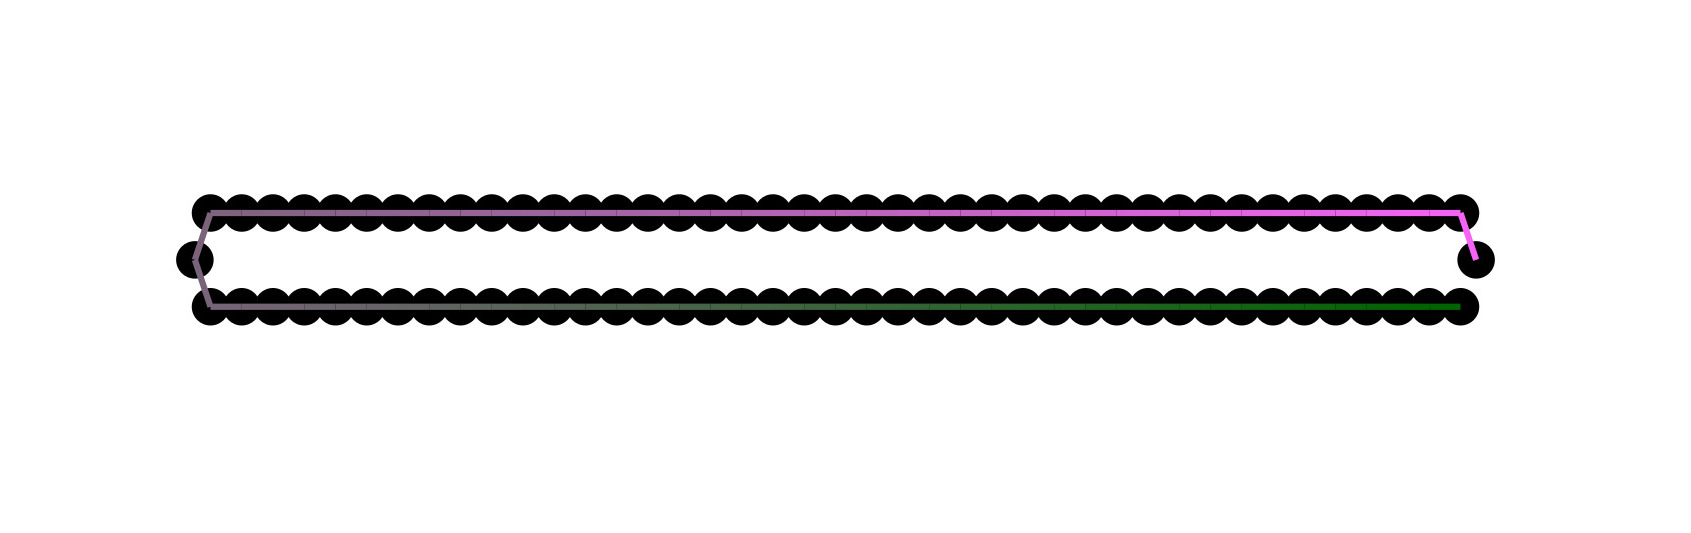
\includegraphics[]{output__wenigerkrumm1__847.4342.jpg} 
    \subsubsection{wenigerkrumm2}
        Das zweite Beispiel wird noch schneller als das erste gelöst. Der erste Startpfad liegt im inneren Punktering und der Algorithmus folgt diesem, bis alle inneren Punkte enthalten sind. Danach wird der dichteste Punkt des äußeren Kreises probiert. Von diesem kann jedoch kein anderer Punkt mehr erreicht werden, da ansonsten die Winkelbedingung nicht erfüllt wäre. Es wird ein Punkt zurück gegangen und der nächst dichteste probiert. Von diesem kann der äußere Ring umlaufen werden. Die unten gezeigt Lösung wird gefunden. \\
        \lstinline{\$: ./bwinf-test --path pfad/zu/wenigerkrumm2.txt 1000} \\
        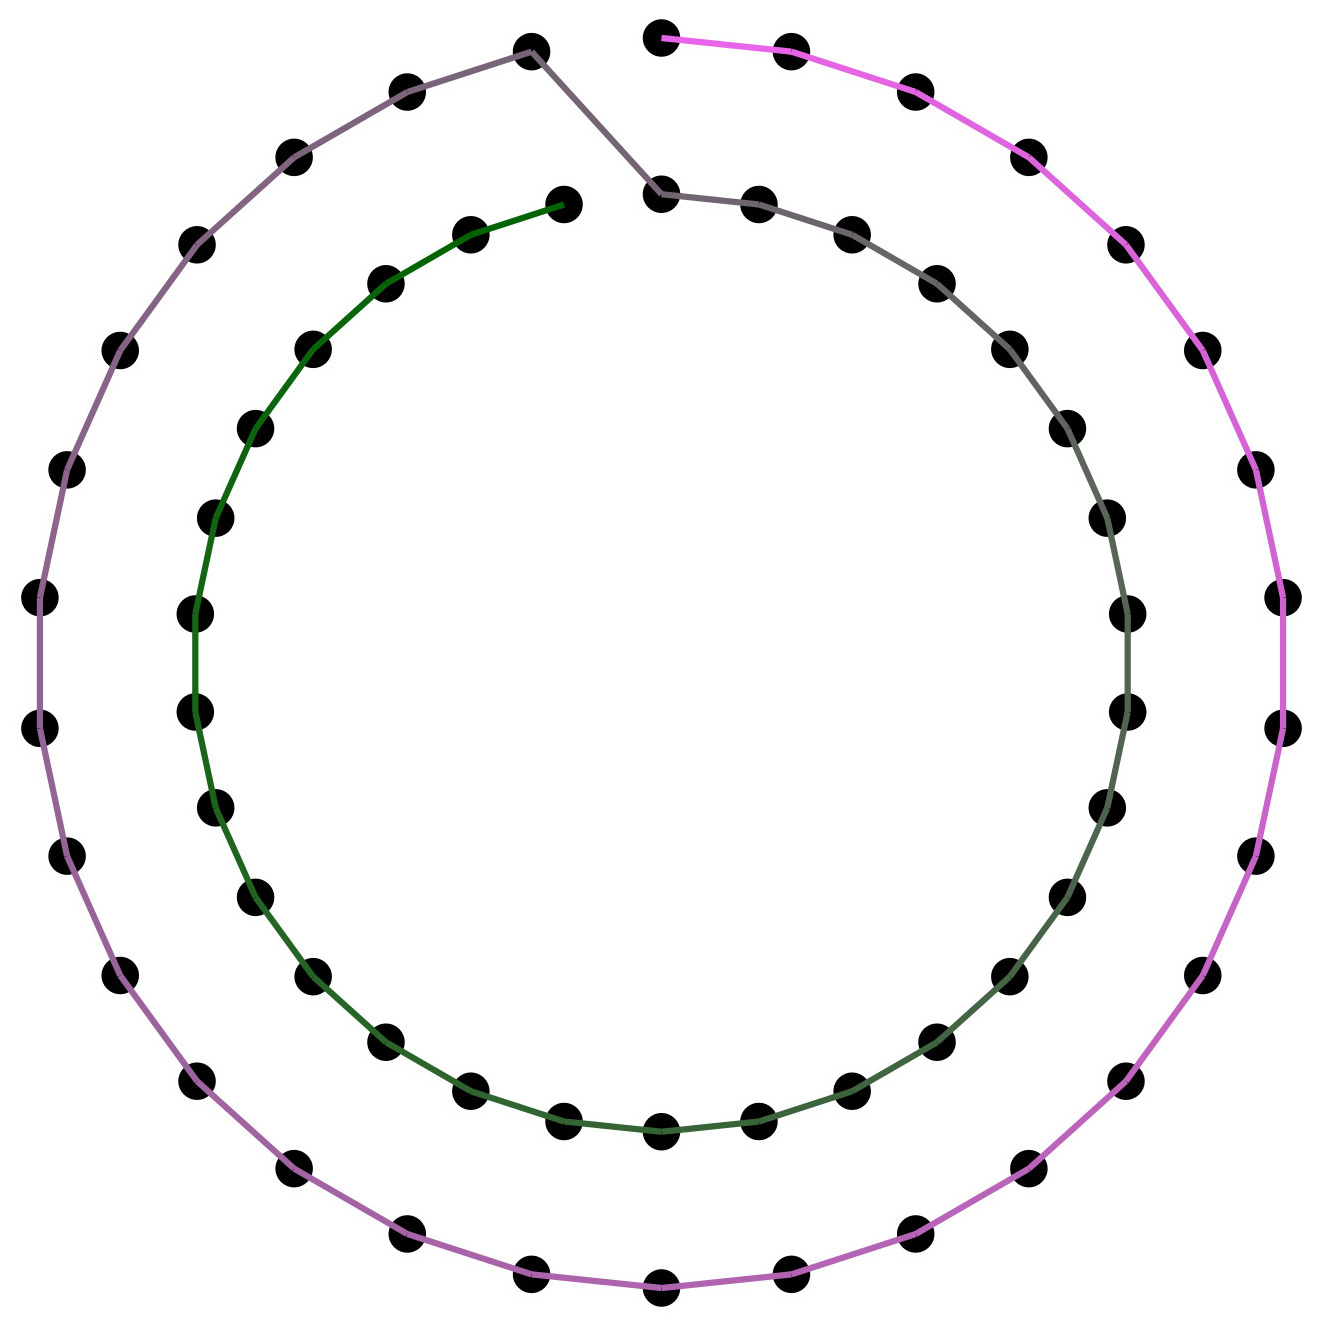
\includegraphics[]{output__wenigerkrumm2__2183.662.jpg} \newpage
    \subsubsection{wenigerkrumm3}
        Das dritte Beispiel wird nicht so gut gelöst wie die vorherigen. Da immer die dichteste Node erreicht werden soll, folgt der Algorithmus nicht den für Menschen offensichtlich kürzeren vorgegebenen Kreisen.\\
        \lstinline{\$: ./bwinf-test --path pfad/zu/wenigerkrumm3.txt 1000} \\
        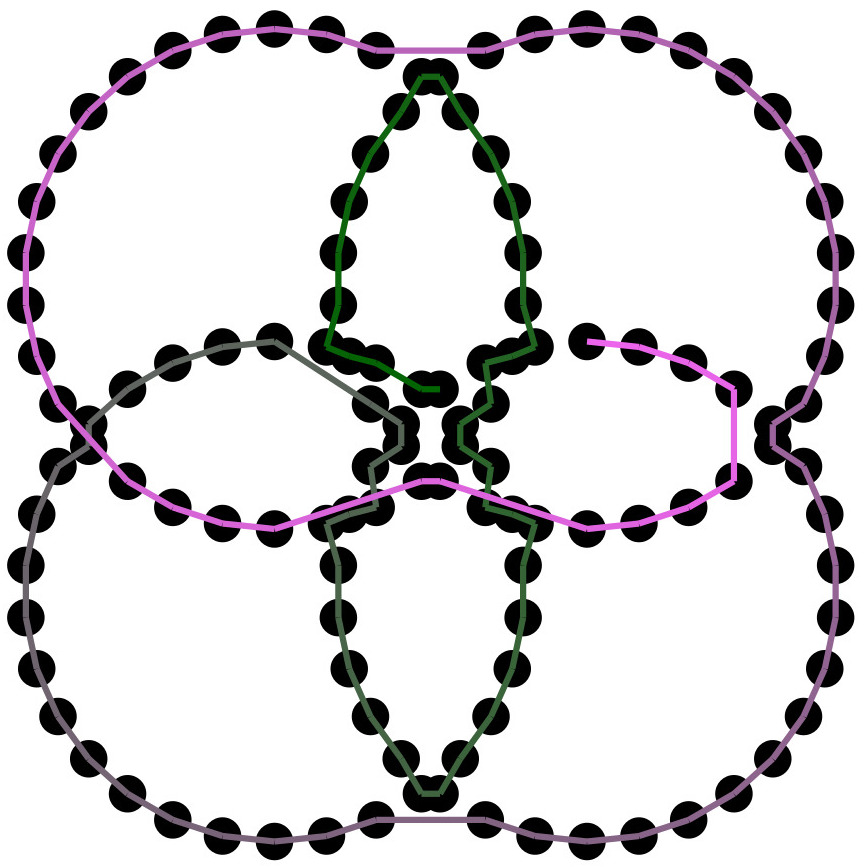
\includegraphics[]{output__wenigerkrumm3__1921.1172.jpg}
    \subsubsection{wenigerkrumm4}
        Beim vierten Beispiel ist es schwieriger Nachzuvollziehen, wie die Lösung erreicht wurde. Da es keinerlei Überschneidungen im Pfad gibt und fast alle Nodes mit ihren dichtesten Nachbarn verbunden sind, handelt es sich aber offensichtlich um eine sehr gute Lösung. Hier wird auch klar wie nützlich das Wechseln der Startposition ist. Bei diesem Beispiel begint der Pfad nähmlich an einer Stelle, welche keine leicht zu identifizierbaren Merkmale hat.\\ 
        \lstinline{\$: ./bwinf-test --path pfad/zu/wenigerkrumm4.txt 1000} \\
        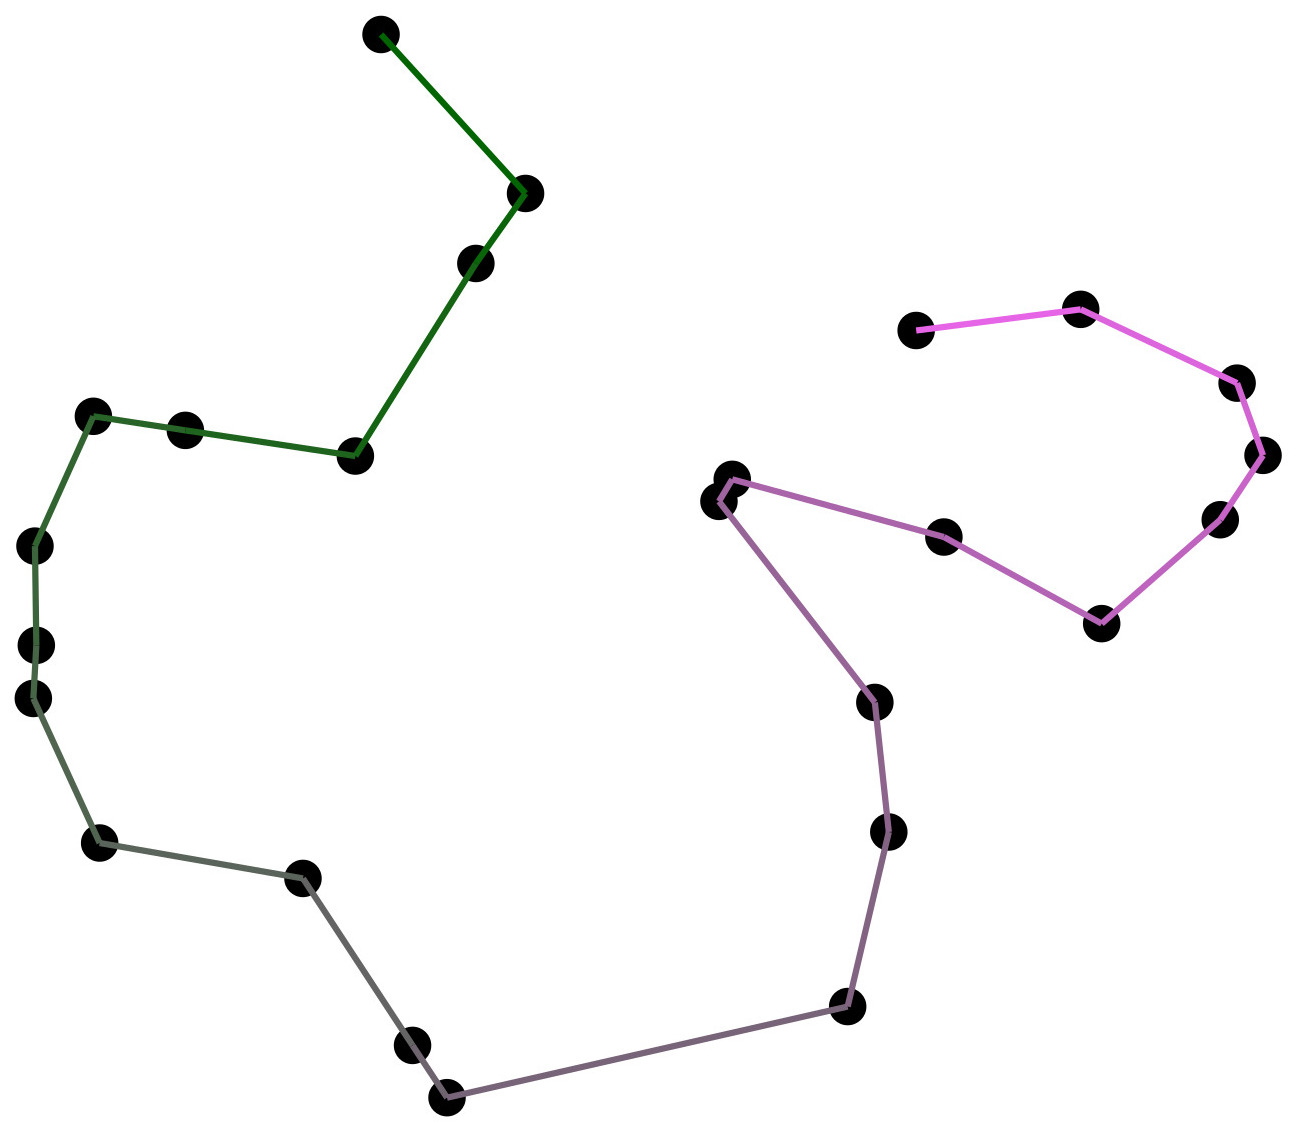
\includegraphics[]{output__wenigerkrumm4__1205.0686.jpg}
    \subsubsection{wenigerkrumm 5 bis 7}
        Die Beispiele 5 bis 7 sind zusammengefasst, da sie alle ähnlich sowohl in ihrem Aufbau als auch ihrer Lösung sind. Es fällt auf, dass sich der Algorithmus mit größeren Netzen schwerer tut. Der Pfad nimmt manchmal große Umwege, um Nodes zu erreichen, welche eigentlich schon früher erreichbar gewesen wären. Es wird deutlich, dass bei diesem Ansatz die Variation in den anfänglichen Teilen des Pfades fehlt. Wenn besonders zu Begin eine Route gewählt wird, die spätere Möglichkeiten verbaut, kann dies nicht mehr korrigiert werden. Eine Möglichkeit diesen Aspekt zu verbessern ist, nachdem eine Lösung gefunden wurde, Abschnitte und einzelne Nodes miteinander zu vertauschen, um so eine schnellere Route zu finden.\\
\begin{enumerate}
    \item
        \lstinline{\$: ./bwinf-test --path pfad/zu/wenigerkrumm5.txt 1000} \\
        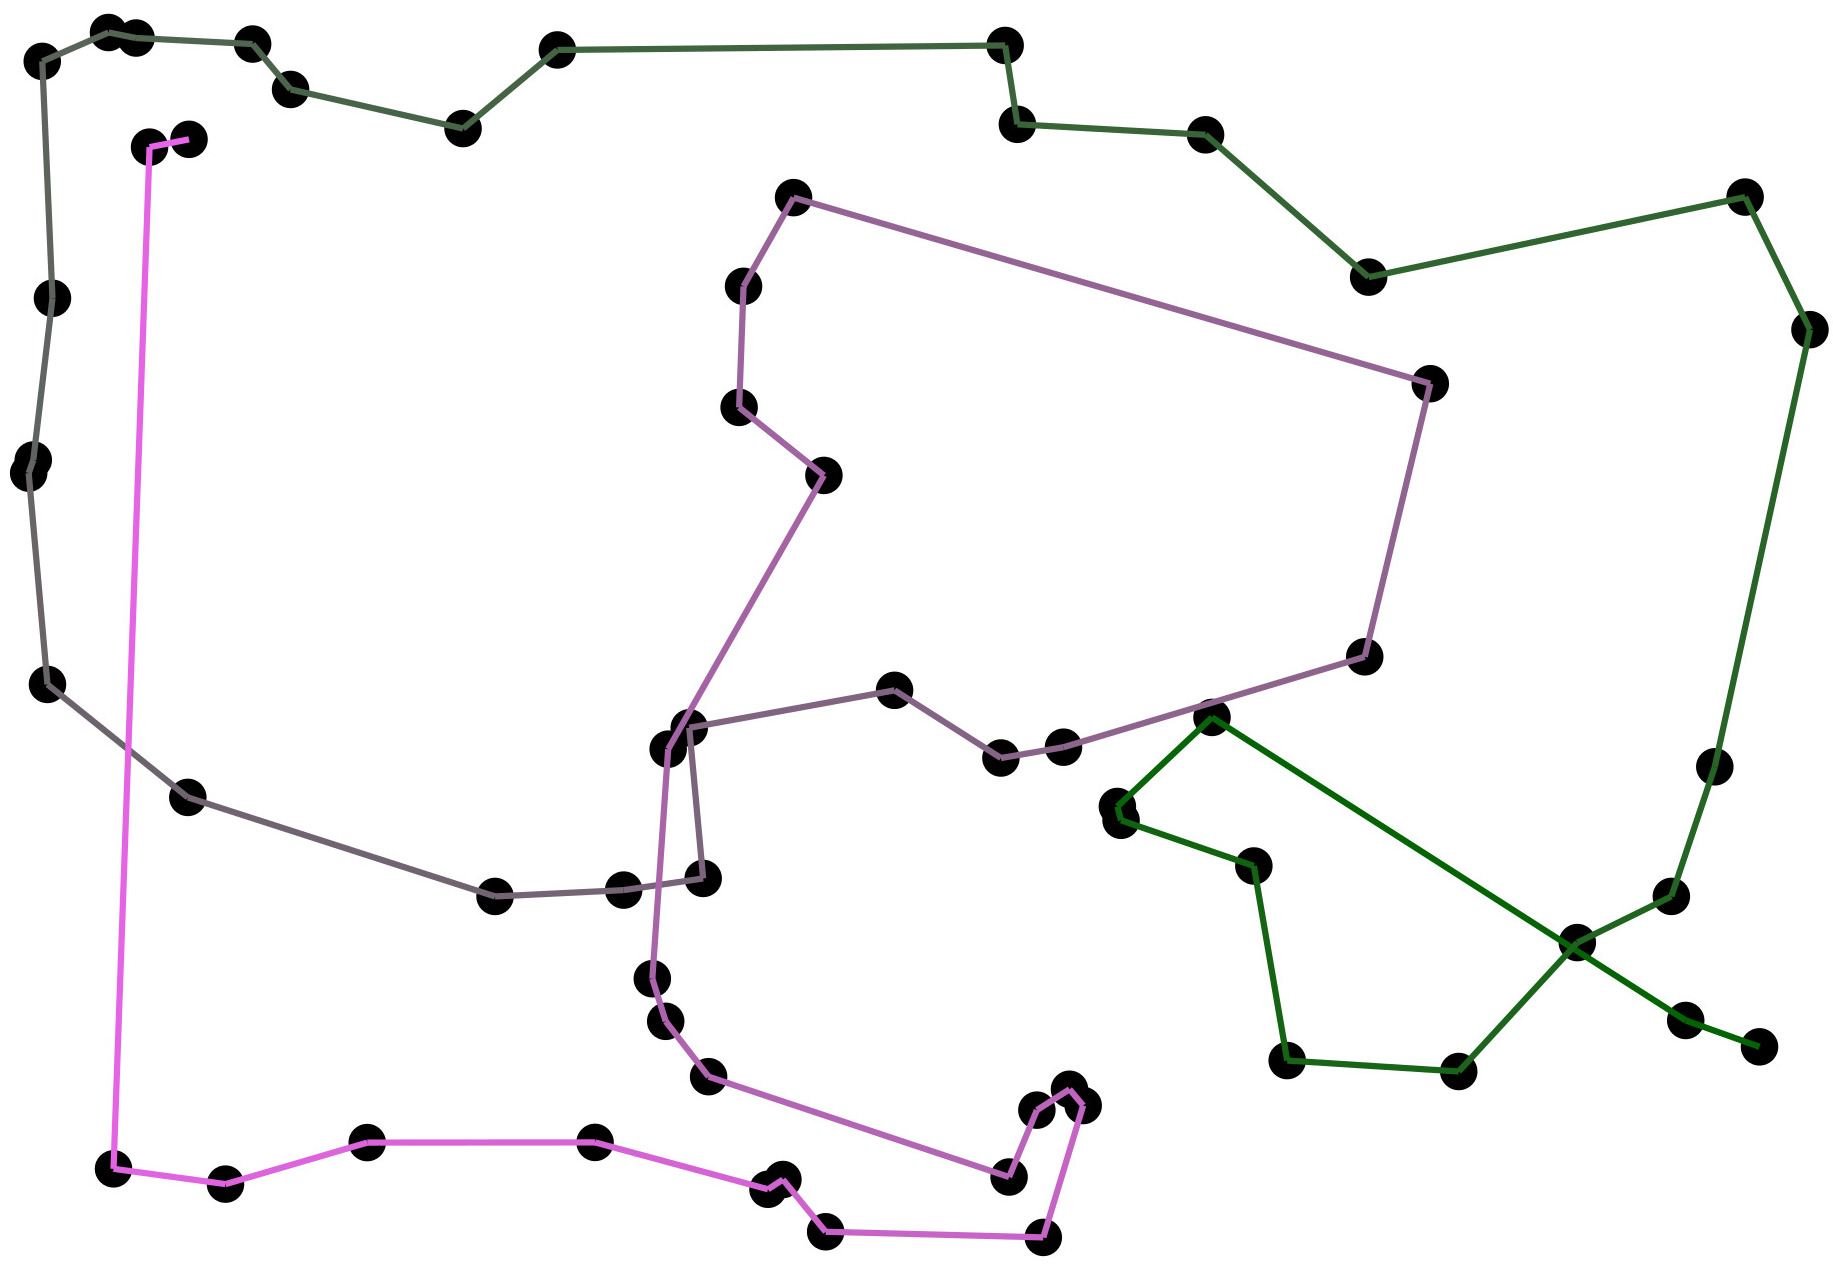
\includegraphics[]{output__wenigerkrumm5__3506.4656.jpg}
    \newpage
    \item 
        \lstinline{\$: ./bwinf-test --path pfad/zu/wenigerkrumm6.txt 1000} \\
        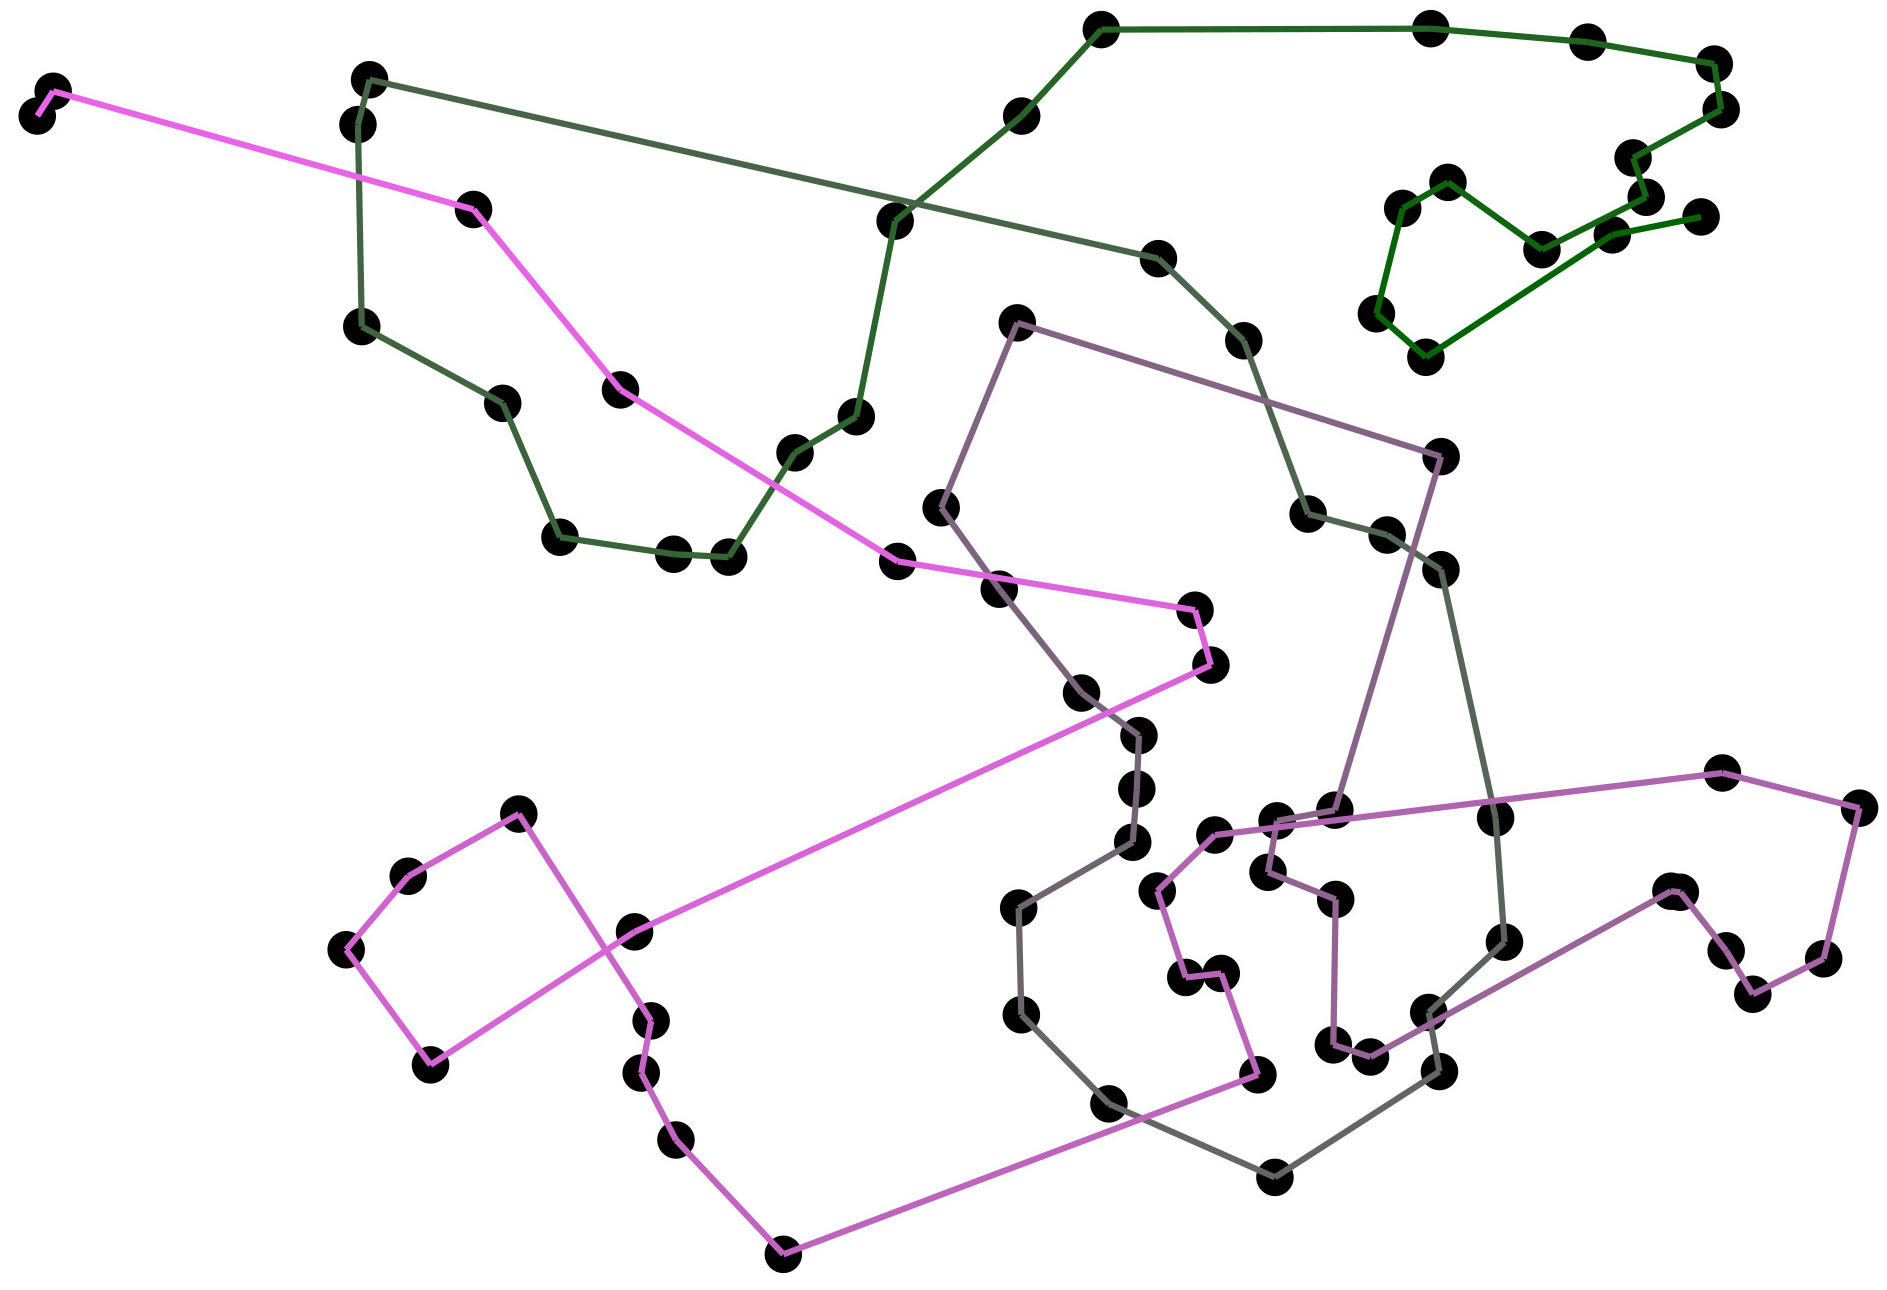
\includegraphics[]{output__wenigerkrumm6__4049.9133.jpg}
    \item 
        \lstinline{\$: ./bwinf-test --path pfad/zu/wenigerkrumm7.txt 1000} \\
        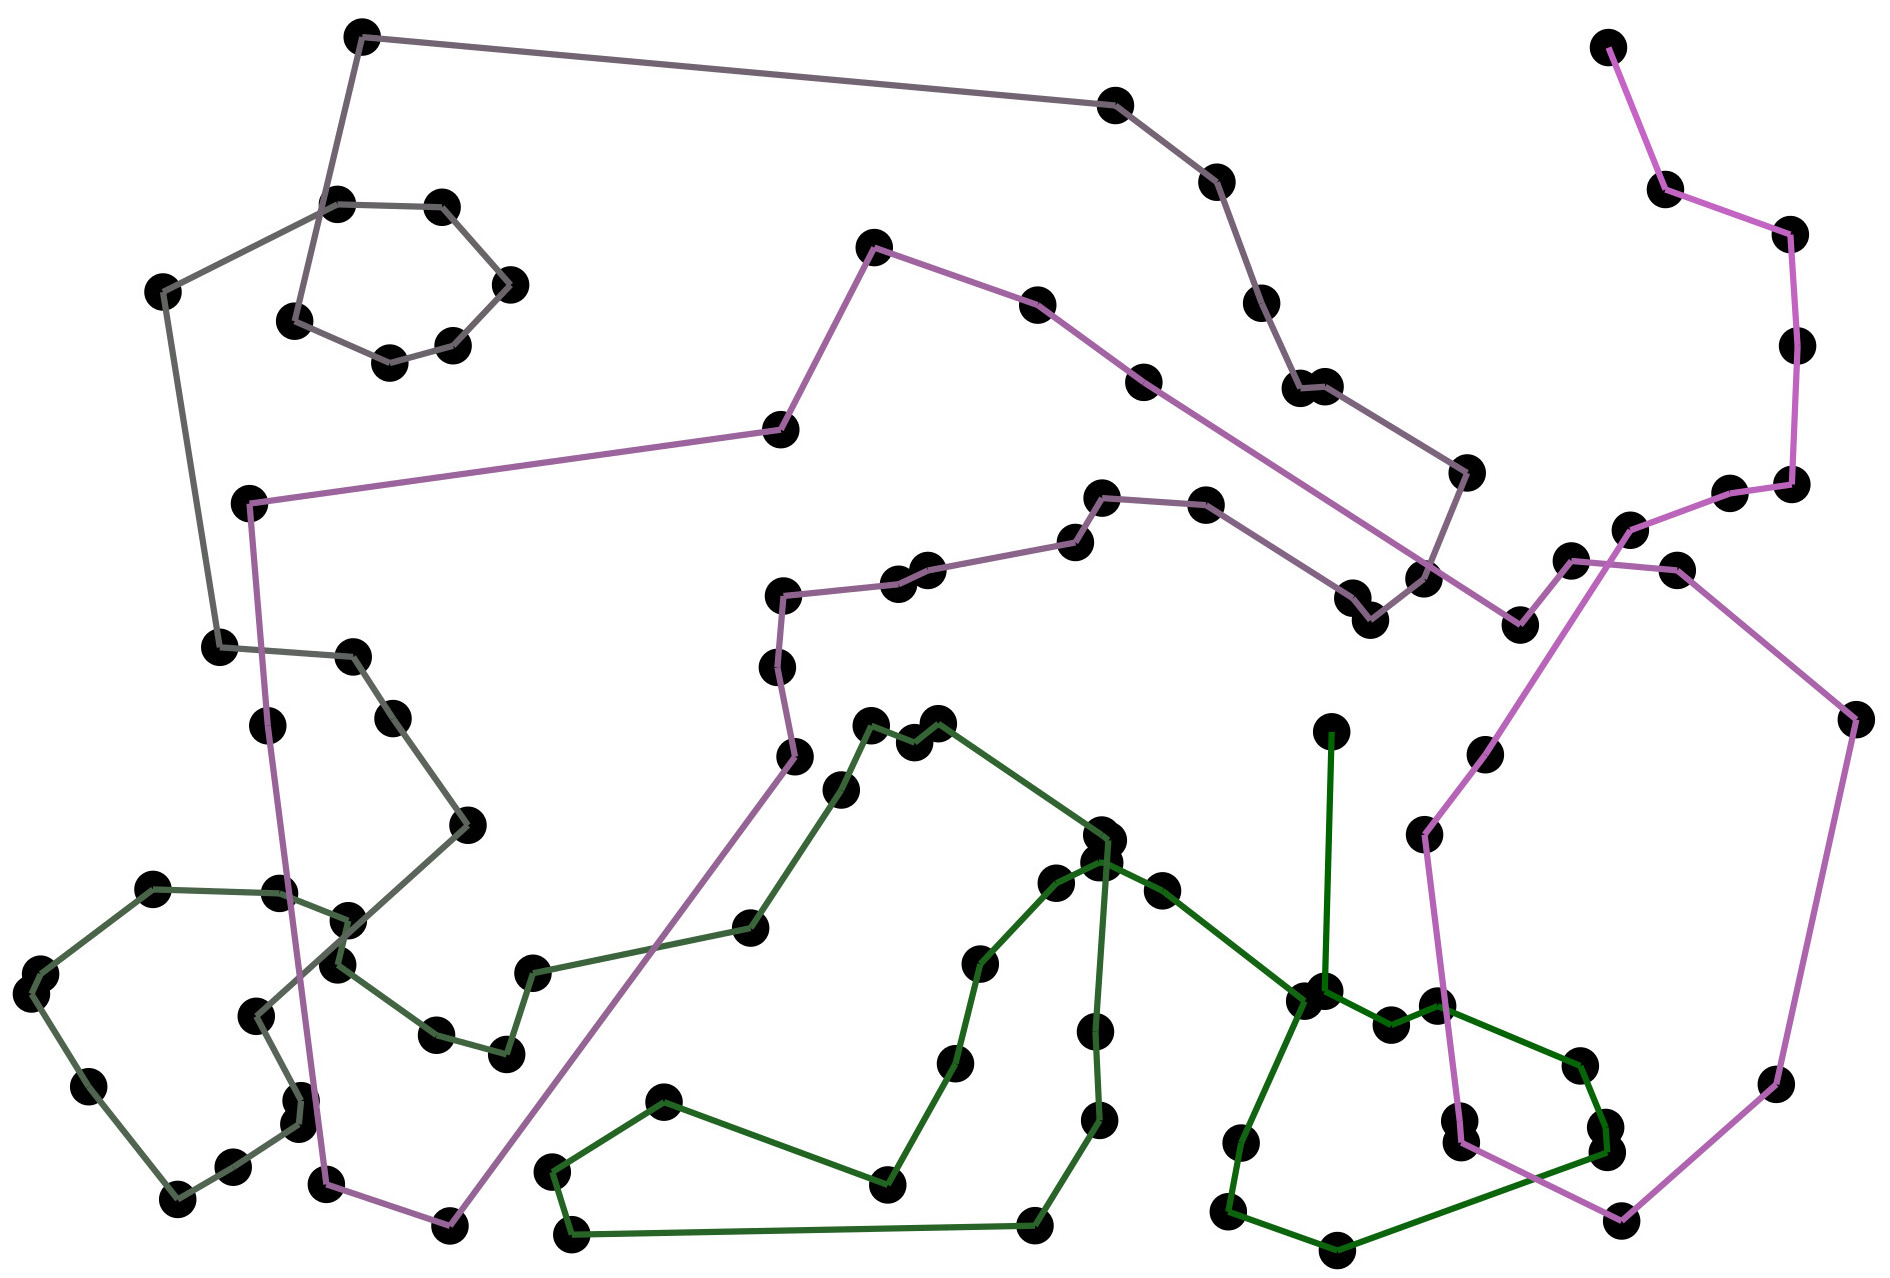
\includegraphics[]{output__wenigerkrumm7__4748.518.jpg}
\end{enumerate}

\newpage
\section{Quellcode}
\lstset{style=boxed}
\begin{lstlisting}[language=Rust]
// Für den eigentlchen Algorithmus irrelevanter Code,
// zum schreiben und lesen von Beispielen und Lösungen
mod input_output_mod;

// Enthält den Node Struct und dessen Funktionen
mod node_mod;

// Funktionen zum lesen und schreiben
use input_output_mod::{read_nodes, render};
// Logging crate 
use log::{debug, info};
use node_mod::Node;
use std::cmp::Ordering;
use std::f32::MAX;
use std::num::NonZeroUsize;
use std::path::PathBuf;
use std::sync::{Arc, Mutex};
// use std::time::Instant;
use std::thread::available_parallelism;
use std::thread::{self, JoinHandle};
use indicatif::{ProgressBar, ProgressStyle};

// Berechnet die Länge Eines Pfades bestehend aus Indexen von Nodes
fn path_len(path: &Vec<usize>, distances: &[Vec<f32>]) -> f32 {
    let mut distance: f32 = 0f32;
    // "rest" enthält jetzt den Pfad bis auf das letzte Element
    let (_last, rest) = path.split_last().unwrap();
    for (i, _node_index) in rest.iter().enumerate() {
        // Für jede Node im path wird die Distanz zur nächsten berechnet
        distance += distances[path[i]][path[i + 1]];
    }
    distance
}

fn calc_angles_distances(nodes: &Vec<Node>) -> 
        (Vec<Vec<Vec<usize>>>, Vec<Vec<f32>>) { 
    // 2d Vector, um alle Distanzen zwischen 2 Nodes zu speichern
    let mut distances: Vec<Vec<f32>> = vec![];
    // 3d Vector, um alle Ergänzungen für 2 Nodes zu speichern
    let mut angles: Vec<Vec<Vec<usize>>> = vec![];
    // Debug Variable, um Menge von einträgen zu zählen
    let mut cache_entries = 0;
    // Es wird zum ersten Mal über jede Node iteriert 
    for (start_node_index, start_node) in nodes.iter().enumerate() {
        // Beide Vectoren werden "2d gemacht"
        distances.push(vec![]);
        angles.push(vec![]);
        for (main_node_index, main_node) in nodes.iter().enumerate() {
            distances[start_node_index].push(start_node.distance(main_node));
            angles[start_node_index].push(vec![]);
            for (end_node_index, end_node) in nodes.iter().enumerate() {
                let angle = main_node.angle(start_node, end_node);
                debug!(
                    "Angle between {:?}, {:?}, {:?} : {:?}", 
                    start_node_index, 
                    main_node_index, 
                    end_node_index, 
                    angle);
                if 90f32 <= angle {
                    angles[start_node_index][main_node_index].push(end_node_index);
                    cache_entries += 1;
                }
            }
            // Die erstellte Liste wird nach Distanz zur mittleren Node sortiert
            angles[start_node_index][main_node_index].sort_by(|a, b| {
                let node_a = &nodes[*a]; 
                let node_b = &nodes[*b];
                // Distanz wird ausgerechnet
                let node_a_distance = main_node.distance(node_a);
                let node_b_distance = main_node.distance(node_b);
    
                // Distanz wird mit Wert zum vergleichen gleichgesetzt
                let val_a = node_a_distance;
                let val_b = node_b_distance;
                if val_a < val_b {
                    Ordering::Less
                } else if val_a == val_b {
                    Ordering::Equal
                } else {
                    Ordering::Greater
                }
            });
        }
    }
    info!("Cache entries count: {}", cache_entries);
    debug!("Cached entries: {:?}", angles);
    debug!("Cached distances: {:?}", distances);
    (angles, distances)
}

fn sort_paths(tasks: &mut Vec<Vec<usize>>, distances: &Vec<Vec<f32>>) {
    tasks.sort_by(|a, b| {
        let val_a = path_len(&a, distances);
        let val_b = path_len(&b, distances);
        if val_a > val_b {
            Ordering::Less
        } else if val_a == val_b {
            Ordering::Equal
        } else {
            Ordering::Greater
        }
    });
}

// Gibt alle Kombinationen aus 3 unterschiedlichen Nodes nach länge sortiert zurück
fn generate_start_paths(
    angles: &Vec<Vec<Vec<usize>>>,
    distances: &Vec<Vec<f32>>,
) -> Vec<Vec<usize>> {
    let mut paths: Vec<Vec<usize>> = vec![];
    for (first_node_index, second_node_indices) in 
            angles.iter().enumerate() {
        for (second_node_index, third_node_indices) in 
                second_node_indices.iter().enumerate() {
            for valid_third_node_index in 
                    third_node_indices.iter() {
                if first_node_index != second_node_index
                    && second_node_index != *valid_third_node_index
                    && first_node_index != *valid_third_node_index
                {
                    let path = vec![
                        first_node_index, 
                        second_node_index, 
                        *valid_third_node_index
                    ];
                    paths.push(path);
                }
            }
        }
    }
    sort_paths(&mut paths, distances);
    debug!("Start paths: {:?}", paths);
    info!("Generated {} start paths", paths.len());
    paths
}

fn indices_to_nodes(
        nodes: Vec<Node>, 
        indices_path: &Vec<usize>) -> Vec<Node> {
    let mut node_path: Vec<Node> = vec![];
    for i in indices_path {
        node_path.push(nodes[*i]);
    }
    node_path
}

fn solve_recursive(
    path: &mut Vec<usize>, 
    path_length: f32,
    nodes: &Vec<Node>, 
    angles: &Vec<Vec<Vec<usize>>>, 
    distances: &Vec<Vec<f32>>, 
    best_solution: &mut Arc<Mutex<Vec<usize>>>, 
    best_solution_length: &mut Arc<Mutex<f32>>,
    input_file_name: &String, 
    iterations: &mut u64,
    max_iterations: &u64,
) {
    // Jeder Aufruf der Funktion erhöht den iterationszähler um 1 
    *iterations += 1;
    // ========== ANFANG DER ABBRUCHBEDINGUNGEN ============================
    // Die Länge der besten bekannten Lösung ist über alle Threads geteilt.
    // Deshalb wird die Variable zuerst "gelocked", 
    // um andere Threads am Verändern zu hindern.
    let mut sol_len = best_solution_length.lock().unwrap();
    // Abgebrochen wird, wenn die maximale Menge an Iterationen 
    // erreicht oder die Länge des eigenen Pfades größer 
    // als die der kürzesten bekannten Lösung ist.
    if *iterations > *max_iterations || path_length >= *sol_len {return};
    // Wenn es so viele Einträge im Pfad, wie Nodes gibt, wurde eine Lösung 
    // gefunden, wird sie als neue gespeichert und die Funktion abgebrochen.
    if path.len() == nodes.len() {
        // Auch die beste Lösung wird "gelocked"
        let mut best_solution_lock = 
        	best_solution.lock().unwrap_or_else(|e|panic!("{}", e));
        // Der aktuelle Pfad wird in die Stelle der besten Lösung geklont
        path.clone_into(&mut best_solution_lock);
        // Die Länge der besten Lösung wird aktuallisiert 
        *sol_len = path_length;
        // Die Lösung wird als txt und svg gespeichert
        render(
            nodes, 
            &indices_to_nodes(nodes.clone(), &best_solution_lock), 
            path_length, input_file_name.clone()
        );
        return;
    }
    // Die Länge der besten Lösung wird nicht mehr benötigt
    // und fallen gelasssen, um anderen Threads den Zugriff zu gewähren
    drop(sol_len);
    // ========== ENDE DER ABBRUCHBEDINGUNGEN ============================

    // Alle Möglichen Ergänzungen der letzten zwei Pfadeinträge
    // welche die Winkelbedingung erfüllen,
    // werden nach Distanz sortiert in "options" gespeichert
    let mut options: Vec<usize> = 
    	angles[path[path.len() - 2]][path[path.len() - 1]].clone();
    // Es werden nur die behalten, welche nicht im Pfad enthalten sind
    options.retain(|x| !path.contains(x));

    // Jede dieser Nodes
    for i in options {
        // Wird zum Pfad hinzugefügt
        path.push(i);
        // Die zusätzliche Länge wird berechnet
        let add_length = distances[path[path.len() - 2]][path[path.len() - 1]];
        // Der veränderte Pfad wird mit den anderen Parametern weitergegeben
        solve_recursive(
            path, 
            path_length + add_length, 
            nodes, 
            angles, 
            distances, 
            best_solution, 
            best_solution_length, 
            input_file_name, 
            iterations, 
            max_iterations,
        ); 
        // Nachdem das finden der Lösungen dieses Teilbaumes abgeschlossen ist, 
        // werden die Veränderungen zum Pfad wieder rückgängig gemacht 
        path.pop().unwrap();
    }
}

fn main() {
    env_logger::init();

    assert!(PathBuf::from("./outputs/txt/").is_dir(), 
    "Txt Ordner nicht gefunden. Bitte sicherstellen, dass der Pfad ./outputs/txt/ valide ist");
    assert!(PathBuf::from("./outputs/svg/").is_dir(), 
    "Svg Ordner nicht gefunden. Bitte ebenfalls sicherstellen, dass der Pfad ./outputs/svg/ valide ist");

    // Ließt alle Nodes und die Suchlänge ein
    let (nodes, max_iterations, name) = read_nodes();

    // Winkel und Distanzen werden zum schnellen auslesen berechnet
    let (angles, distances) = calc_angles_distances(&nodes);

    // Alle Anfangspfade werden bestimmt
    let generated_paths = generate_start_paths(&angles, &distances);

    // Diese Variablen sind über alle Threads geteilt:
    // Vector mit Startpfaden die noch probiert werden müssen
    let start_paths: Arc<Mutex<Vec<Vec<usize>>>> = 
    	Arc::new(Mutex::new(generated_paths.clone()));
    // Die aktuell beste bekannte Lösung
    let best_solution: Arc<Mutex<Vec<usize>>> = Arc::new(Mutex::new(vec![]));
    // Die Länge der aktuell besten bekannten Lösung
    let best_solution_length: Arc<Mutex<f32>> = Arc::new(Mutex::new(MAX));
    let done_threads: Arc<Mutex<u32>> = Arc::new(Mutex::new(0));

    // Hier werden die handles für die Threads eingetragen werden
    let mut handles: Vec<JoinHandle<()>> = vec![];
    // Bestimmt, wie viele CPU Kerne zur Verfügung stehen
    let total_threads: usize = available_parallelism()
        .unwrap_or(NonZeroUsize::new(1).unwrap()).into();

    // Erstellen der Fortschrittsleiste
    let bar: ProgressBar = ProgressBar::new(generated_paths.len() as u64)
        .with_style(ProgressStyle::with_template(
        "[{elapsed_precise}] {bar:40.cyan/blue} {pos:>7}/{len:7} {msg} (eta: {eta})"
        ).unwrap()
    );
    bar.set_message("Geprüfte Startpfade");
let bar = Arc::new(Mutex::new(bar));

    info!("Starting up {:?} threads", total_threads);
    for _i in 0..(total_threads - 1) {
        // Jeder Thread benötigt Zugriff auf die obigen Variablen.
        // Deshalb werden diese vom Hauptthread in neue mit "l_" 
        // notierte Variablen geklont. 
        // Jede der geteilten Variablen benötigt eine Referenz
        let mut l_best_solution = Arc::clone(&best_solution);
        let mut l_best_solution_length = Arc::clone(&best_solution_length);
        let l_start_paths = Arc::clone(&start_paths);
        let l_done_threads = Arc::clone(&done_threads);
        let l_bar = Arc::clone(&bar);

        // Konstante Werte werden geklont
        let l_nodes = nodes.clone();
        let l_angles = angles.clone();
        let l_distances = distances.clone();
        let l_name = name.clone();
        let l_max_iterations = max_iterations.clone();
        let l_total_tasks = generated_paths.len();

        // Der neue Thread wird gestartet.
        // Die obigen "l_" Variablen ziehen in den Thread um, 
        // wenn sie Referenziert werden.
        let handle = thread::spawn(move || {
            info!("Started thread {:?}", thread::current().id());
            loop {
                let mut todo = l_start_paths.lock().unwrap();
                // Falls noch ein ungeprüfter Startpfad existiert
                if let Some(mut l_start_path) = todo.pop() {
                    let thread_number = todo.len();
                    drop(todo);
                    let l_path_length = path_len(&l_start_path, &l_distances);
                    let mut l_iterations = 0;
                    // Finde alle Lösungen
                    solve_recursive(
                        &mut l_start_path, 
                        l_path_length, &l_nodes, 
                        &l_angles, &l_distances, 
                        &mut l_best_solution, 
                        &mut l_best_solution_length, 
                        &l_name, 
                        &mut l_iterations, 
                        &l_max_iterations
                    );
                    // Debug und ausgabe (irrelevant)
                    let mut done = l_done_threads.lock().unwrap();
                    let bar = l_bar.lock().unwrap();
                    bar.inc(1);
                    drop(bar);
                    *done += 1;
                    debug!(
                        "Thread {:?} finished path with priority {:?}  {:?}/{:?}",
                        thread::current().id(), 
                        thread_number, 
                        done, 
                        l_total_tasks
                    );
                    drop(done);
                } else {
                    info!("Thread {:?} returned", thread::current().id());
                    // Beende die Schleife und damit den Thread,
                    // wenn alle Startpfade probiert worden sind
                    break;
                }
            }
        });
        // Thread handle wird gespeichert
        handles.push(handle);
    }
    // Iteriert über alle Threadhandles und wartet bis sie fertig sind
    while let Some(handle) = handles.pop() {
        handle.join().unwrap();
    }
    bar.lock().unwrap().finish();

    let final_solution = best_solution.lock().unwrap();
    // Stellt die gefundene Lösung dar
    if !final_solution.is_empty() {
        render(
            &nodes, 
            &indices_to_nodes(nodes.clone(), &final_solution), 
            path_len(&final_solution, &distances), 
            name
        );
    }
}
\end{lstlisting}

\end{document}
